\documentclass[conference]{IEEEtran}
\usepackage[T1]{fontenc}
\usepackage{graphicx}
\usepackage{booktabs}
\usepackage{amsmath}
\usepackage{cite}
\usepackage{url}
\usepackage{microtype}

\begin{document}

\title{Cropping Football Matches to Vertical Format\\for Mobile Devices Using Machine Learning\thanks{Polish title: \emph{Kadrowanie Mecz\'ow Pi\l{}karskich do Formatu Pionowego na Urz\k{a}dzenia Mobilne z Wykorzystaniem Uczenia Maszynowego}.}}

\author{\IEEEauthorblockN{Rados\l{}aw D\k{a}bkowski}
\IEEEauthorblockA{Redge Technologies\\
radoslaw.dabkowski@redge.com}}

\maketitle

\begin{abstract}
Football broadcasts are produced in 16:9, but much of their audience watches on phones in portrait mode. We study how well small learned models can place a 9:16 crop window over a football broadcast frame, first from player positions alone and then with the ball. On the football videos of SportsMOT, ResNet-18, MobileNetV3 and MobileNetV4-Small networks that predict a player-density histogram and pick the window covering most of it keep $51.8\%$ of the players in the crop on 15 held-out videos (fixed centre crop: $38.2\%$, oracle: $56.1\%$), while direct regression of the crop centre is clearly worse ($42.8\%$). On SoccerNet SN-Tracking-2023 (49 test clips) we add a ResNet-18 heatmap ball detector with a lightweight tracker and a policy that selects the window containing the ball and covering most players. The ball is within $38$\,px (in 1080p) of its true position in $77\%$ of the frames where it is visible, against $60\%$ for a fine-tuned YOLO11n with the same tracker; the resulting crop contains the ball in $89\%$ of those frames and $43.6\%$ of the players, compared with $53\%$ and $39\%$ for a fixed centre crop and $40\%$ and $58\%$ for a players-only crop. Temporal smoothing lowers jitter by roughly a factor of three at a cost of one to four points of coverage. The reference crops are derived from annotations, not from a human camera operator, so the results measure agreement with an annotation-based proxy.
\end{abstract}

\begin{IEEEkeywords}
video retargeting, automatic cropping, football, ball tracking, sports video, lightweight CNN, ResNet-18, SportsMOT, SoccerNet
\end{IEEEkeywords}

\section{Introduction}
Football is broadcast in 16:9, whereas a large share of viewers now watch short clips and highlights on phones held in portrait mode. Showing the full frame on a 9:16 screen wastes more than two thirds of the display and shrinks the players to a few pixels. Cropping a 9:16 window out of the 16:9 frame (a window only $31.6\%$ of the frame width) fixes the scale but raises a new problem: the window has to follow the action, and it has to do so smoothly, because a jumping virtual camera is unpleasant to watch.

Manual ``pan and scan'' is expensive, so we ask how far small learned models can automate it. We study \emph{where to place the crop} first from the positions of the players alone, which is robust, and then with the ball, which viewers follow but which is only a few pixels wide in broadcast footage. We make the following contributions:
\begin{itemize}
\item a protocol for evaluating 9:16 cropping of football video on the football part of SportsMOT, with a player-based oracle window and three metrics (players kept in the crop, centre error, temporal jitter);
\item a comparison of ResNet-18 and mobile-class regressors that predict either the crop centre or a player-density histogram directly from the frame, against a detector-plus-rule pipeline (YOLO11n) and simple geometric baselines;
\item a ResNet-18 heatmap ball detector, a single-ball tracker and a ball-aware crop policy, evaluated on SoccerNet SN-Tracking-2023 against YOLO11n, with ball-in-crop as the main metric;
\item a measurement of the accuracy/latency trade-off on a 4\,GB laptop GPU and on CPU, relevant for on-device deployment.
\end{itemize}

\section{Related Work}
\textbf{Video retargeting.} Automatic ``pan and scan'' dates back to saliency-driven retargeting of video to other aspect ratios~\cite{liu2006}, and is available in production tools such as Google's AutoFlip, which combines face and object detection with a smoothed camera path. Sports differ from generic content because the relevant region is defined by the game rather than by salient objects.

\textbf{Datasets.} SoccerNet~\cite{giancola2018} and its tracking extension~\cite{cioppa2022} provide large-scale annotated football video. SportsMOT~\cite{cui2023} is a multi-object tracking benchmark of 240 videos of basketball, football and volleyball with box and identity annotations for every player; we use its football videos. It contains no ball annotation, so our reference crop is derived from the players.

\textbf{Ball detection and tracking.} The ball is tiny, fast and often occluded; heatmap-based detectors such as CenterNet~\cite{zhou2019} and TrackNet~\cite{huang2019}, trained with a focal loss~\cite{lin2017}, are common choices. SN-Tracking-2023 annotates the ball in every frame in which it is visible, which makes it usable for training and for evaluating ball-driven cropping.

\textbf{Lightweight networks.} ResNet-18~\cite{he2016} is a standard compact backbone; MobileNetV3~\cite{howard2019} and MobileNetV4~\cite{qin2024} target mobile hardware. YOLO11~\cite{yolo11} and CenterNet~\cite{zhou2019} are compact detectors that can supply player positions for a rule-based crop.

\section{Method}
\subsection{Problem and reference crop}
Let a frame have width $W$ and let the crop window have width $w=\tfrac{9}{16}\cdot\tfrac{9}{16}\,W\approx0.316\,W$ (a 9:16 window of full frame height). The task is to choose the horizontal window centre $c_t\in[w/2,\,W-w/2]$ for every frame $t$. Because SportsMOT has no human-operated virtual camera, we define the \emph{oracle} centre $c^\star_t$ as the centre of the window that contains the most player centres (ties are broken towards the median player position). The oracle is thus a proxy for ``keep the action in view''; it is not a human editor's choice, and it is jumpy by construction since it ignores time.

\subsection{Models}
\textbf{Direct models.} A backbone (ResNet-18, MobileNetV3-Large or MobileNetV4-Conv-Small, ImageNet-pretrained) processes a $252\times448$ frame. Features are reduced by a $1{\times}1$ convolution, averaged over the vertical axis to keep only horizontal structure, and passed to one of two heads:
\begin{itemize}
\item \emph{reg}: a small MLP regressing the centre $c_t/W$ (L1 loss against $c^\star_t$);
\item \emph{hist}: a 1-D convolution producing logits of a 64-bin histogram of player $x$-positions, trained with KL divergence to the (lightly smoothed) ground-truth histogram. At inference the crop centre is the window covering the largest predicted mass, so the model reproduces the oracle rule on its own prediction.
\end{itemize}
A \emph{two-frame} variant feeds the frame and its difference to the frame $0.24$\,s earlier (6 input channels, extra weights initialised at zero) to expose motion.

\textbf{Detector + rule.} YOLO11n~\cite{yolo11} detects players at $640$\,px width; the crop centre is the oracle rule applied to the detected player centres (confidence $\ge0.25$). We evaluate the COCO-pretrained model with the \emph{person} class (zero-shot) and a version fine-tuned on SportsMOT football.

\textbf{Baselines.} Fixed frame centre; mean and median of the \emph{ground-truth} player positions (not available at test time, so they bound rule-based methods that use perfect detections).

\subsection{Temporal post-processing}
The raw per-frame centres are post-processed per video: \emph{raw}; \emph{ema}, exponential smoothing $\hat c_t=\alpha c_t+(1-\alpha)\hat c_{t-1}$ with $\alpha=0.5$; and \emph{ema+limit}, the same with the per-sample pan step clipped to $2\%$ of the frame width. Samples are $0.12$\,s apart (8.3\,fps).

\subsection{Ball detection, tracking and ball-aware policy}
\textbf{Ball network.} A ResNet-18 encoder (ImageNet-pretrained) with a light top-down decoder (lateral $1{\times}1$ convolutions on the four stages, nearest-neighbour upsampling and addition) outputs a stride-4 heatmap of ball-centre probability on a $504{\times}896$ frame. It is trained with the CenterNet focal loss~\cite{zhou2019} on a Gaussian target ($\sigma=1.5$ cells) using random $288{\times}512$ crops of the training frames (the ball is inside the crop with probability $0.75$), horizontal flips and brightness/contrast jitter. At test time the full frame is processed and the five strongest local maxima are kept as candidates.

\textbf{Tracker.} A single-ball tracker runs per clip over the samples (0.12\,s apart). For each sample it picks the candidate above a score threshold maximising score minus a penalty proportional to the distance from the last position; jumps farther than a gate (25\% of the frame width, growing with the time since the last confirmation) to candidates with score below 0.8 are rejected, and the last position is held for a few samples when nothing is accepted. The threshold and the hold length are selected on the validation clips. \emph{Static-overlay suppression} removes candidates that fall in the same image cell in more than 40\% of a clip's samples (logos, score graphics); it uses whole-clip statistics and is therefore offline.

\textbf{Ball-aware policy.} Given a predicted player-density histogram and a ball estimate, the crop is the window that contains the ball (with a margin of $3\%$ of the frame width from the window edge when possible) and covers the largest predicted player mass, ties broken towards the ball; without a ball estimate the densest-player window is used. The reference (oracle) crop is defined in the same way from the ground-truth ball and players. We also evaluate a 2-class (player, ball) YOLO11n whose detections feed the same tracker and policy.

\section{Experimental Setup}
\textbf{Data.} The labelled football videos in SportsMOT are 15 training and 15 validation sequences ($1280{\times}720$, 25\,fps, 450--1\,325 frames each); the test labels are not public. We train on 12 of the official training sequences, select models on the remaining 3, and report on the 15 official validation sequences, which are never used for any decision. Every third frame is kept, giving 2\,801 / 879 / 2\,994 frames (train / validation / test). The data are used under their CC BY-NC 4.0 licence for research only.

\textbf{SN-Tracking-2023.} For the ball experiments we use SoccerNet SN-Tracking-2023, 30\,s broadcast clips ($1920{\times}1080$, 25\,fps) with box annotations of all players, referees and the ball. The official training clips are split into 51 for training and 6 for validation; the 49 official test clips are used for the reported results. Frames are downscaled to $896{\times}504$; every fourth frame is kept for training (9\,588 frames) and validation (1\,128), every third for testing (12\,250). The ball is annotated in $92.0\%$ of the test frames; ball-in-crop is computed on these frames, players-in-crop on all frames. Players are the annotated players and goalkeepers. The data are used for research only, under the SoccerNet terms.

\textbf{Metrics.} \emph{Players in crop}: mean fraction of players whose box centre lies inside the window (higher is better; because the window covers only $31.6\%$ of the width the oracle itself cannot reach 100\%). \emph{Centre MAE}: mean $|c_t-c^\star_t|/W$. \emph{Jitter}: mean $|c_t-c_{t-1}|/W$ between consecutive samples, a proxy for visual stability. \emph{Ball in crop}: fraction of ball-visible frames in which the ball centre is inside the window. \emph{Ball recall / precision}: share of ball-visible frames (recall), respectively of frames with an estimate (precision), in which the estimated ball is within $2\%$ of the frame width ($\approx38$\,px at 1080p) of the annotated centre. We also report parameters and median single-frame latency on an NVIDIA GTX\,1650 (4\,GB, FP32) and on CPU (4 threads, 12-core laptop).

\textbf{Training.} AdamW~\cite{loshchilov2019} (lr $5{\cdot}10^{-4}$, weight decay $10^{-2}$, one-cycle schedule), batch 24, at most 20 epochs with early stopping on validation players-in-crop, random horizontal flips (the target is mirrored accordingly) and brightness/contrast jitter. Mixed precision was disabled because it was about four times slower on this GPU. YOLO11n is fine-tuned for at most 25\,minutes at $640$\,px. The ball network is trained for 10 epochs of 6\,000 crops (about 18 minutes), the SN-trained player model for at most 15 minutes and the 2-class YOLO11n for 35 minutes at $896$\,px. All runs are single-seed unless stated.

\section{Results}
\subsection{Test-set comparison}
Table~\ref{tab:main} reports the 15 held-out videos (2\,994 frames). Each cell pair is raw / smoothed (EMA with pan-speed limit) for players in crop and jitter; centre MAE is for raw predictions.

\begin{table*}[t]
\centering
\caption{Held-out test results (15 SportsMOT football videos). Players in crop and jitter are given for raw predictions and after \emph{ema+limit}; centre MAE and jitter in \% of frame width. Latency is for one $252{\times}448$ frame (YOLO11n: $640{\times}360$), batch 1. Baselines and the oracle use ground-truth player positions. Rows below the rule are sorted by smoothed players in crop.}
\label{tab:main}
\begin{tabular}{lrrrrrrrr}
\toprule
Method & Params [M] & GPU [ms] & CPU [ms] & \multicolumn{2}{c}{Players in crop [\%]} & MAE [\%] & \multicolumn{2}{c}{Jitter [\%]}\\
 & & & & raw & smooth & raw & raw & smooth \\
\midrule
Fixed centre & -- & -- & -- & 38.2 & 38.2 & 12.9 & 0.0 & 0.0 \\
Mean of players (GT) & -- & -- & -- & 41.7 & 41.7 & 9.2 & 1.3 & 0.7 \\
Median of players (GT) & -- & -- & -- & 44.7 & 44.3 & 6.1 & 1.4 & 0.9 \\
Oracle (GT densest window) & -- & -- & -- & 56.1 & 48.4 & 0.0 & 2.7 & 1.2 \\
\midrule
ResNet-18 hist, 2-frame & 11.3 & 5.0 & 34.4 & 51.9 & 48.1 & 8.9 & 4.4 & 1.3 \\
MobileNetV3 hist & 3.1 & 3.7 & 14.7 & 51.7 & 48.0 & 9.3 & 5.1 & 1.3 \\
ResNet-18 hist (seed 2) & 11.2 & 4.8 & 28.6 & 51.7 & 48.0 & 9.2 & 4.4 & 1.3 \\
ResNet-18 hist & 11.2 & 4.8 & 31.8 & 51.8 & 47.9 & 9.2 & 4.3 & 1.3 \\
ResNet-18 hist (seed 1) & 11.2 & 4.8 & 33.0 & 51.3 & 47.2 & 10.1 & 4.8 & 1.4 \\
YOLO11n (fine-tuned) + rule & 2.6 & 5.4 & 21.6 & 53.7 & 47.2 & 6.0 & 5.7 & 1.3 \\
MobileNetV4-S hist & 1.4 & 3.0 & 8.0 & 51.1 & 47.2 & 9.8 & 4.8 & 1.3 \\
YOLO11n (COCO, zero-shot) + rule & 2.6 & 5.5 & 22.0 & 52.6 & 46.4 & 6.7 & 5.9 & 1.4 \\
ResNet-18 reg & 11.5 & 4.8 & 33.1 & 42.8 & 42.5 & 9.0 & 2.0 & 1.0 \\
\bottomrule

\end{tabular}
\end{table*}

\textbf{Heads.} The histogram head is far better than regression of the centre: $51.8\%$ against $42.8\%$ of players kept, where the regressor is barely above the fixed-centre baseline ($38.2\%$) and below the median of the true player positions ($44.7\%$). A plausible reason (not tested separately) is that regressing a single number averages the modes of a scene with players on both sides of the pitch, whereas the histogram keeps both modes and lets the window rule pick the denser one. The raw histogram models recover $92$\% of the oracle's coverage ($51.8$ of $56.1$).

\textbf{Backbones and temporal input.} Three seeds of the ResNet-18 histogram model give $51.6\pm0.3\%$ raw and $47.7\pm0.4\%$ smoothed players in crop (mean $\pm$ standard deviation), so differences below about one point are not reliable. The two-frame variant ($51.9$ / $48.1$), MobileNetV3 ($51.7$ / $48.0$) and MobileNetV4-Small ($51.1$ / $47.2$) all fall within or close to this band; we therefore cannot claim that motion input or a larger backbone helps. MobileNetV4-Small has $8\times$ fewer parameters than ResNet-18 and runs in 8\,ms on CPU, against about 32\,ms.

\textbf{Detector pipeline.} Fine-tuned YOLO11n with the window rule reaches the best raw coverage ($53.7\%$) and the lowest centre error ($6.0\%$), presumably because it sees players at higher resolution and the rule is applied to explicit detections. The COCO-pretrained detector without fine-tuning is only one point behind ($52.6\%$). After smoothing, however, the detector pipeline ($47.2\%$) is level with the direct models; it is also about $2.7\times$ slower on CPU than MobileNetV4-Small and its raw jitter is the highest.

\subsection{Smoothing trades coverage for stability}
Raw per-frame centres jump by $4$--$6\%$ of the frame width between samples (0.12\,s), which would be unwatchable. The EMA with a pan-speed limit reduces jitter to $1.3\%$ for all learned models, in line with the smoothed oracle ($1.2\%$), at the price of about $4$ points of coverage. Notably the smoothed oracle itself drops from $56.1\%$ to $48.4\%$: the learned models are therefore close to the best that a causal smoothed camera can achieve under this proxy, and the remaining gap to the raw oracle is the cost of smooth camera motion rather than of model error. Fig.~\ref{fig:traj} shows a typical trajectory and Fig.~\ref{fig:qual} qualitative frames.

\begin{figure}[t]
\centering
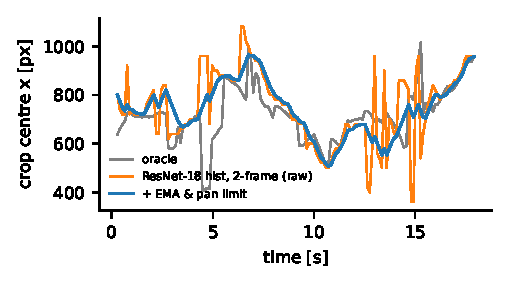
\includegraphics[width=\columnwidth]{figs/trajectory.pdf}
\caption{Crop centre over time for one test video: oracle, raw prediction and smoothed prediction of the best direct model.}
\label{fig:traj}
\end{figure}

\begin{figure*}[t]
\centering
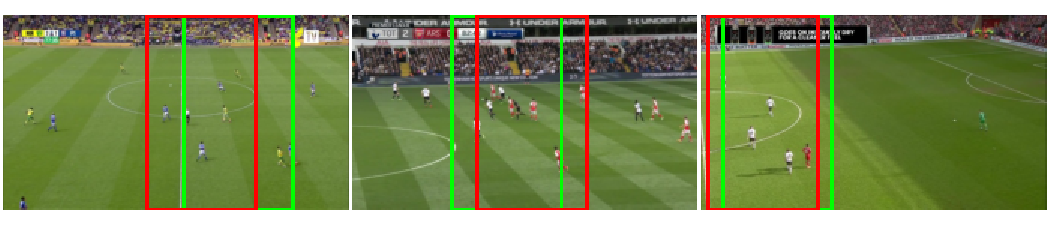
\includegraphics[width=\textwidth]{figs/qualitative.pdf}
\caption{Test frames with the oracle window (green) and the smoothed prediction (red).}
\label{fig:qual}
\end{figure*}

\subsection{Accuracy versus cost}
Fig.~\ref{fig:tradeoff} plots smoothed coverage against CPU latency. All direct models and the detector lie within about one point of each other while spanning a factor of four in latency, so the cheapest model dominates. Median single-frame GPU times of $3$--$6$\,ms and CPU times of $8$--$34$\,ms leave ample margin for real-time use at 8--25 fps, and the cropping decision could be evaluated at a lower rate than the video.

\begin{figure}[t]
\centering
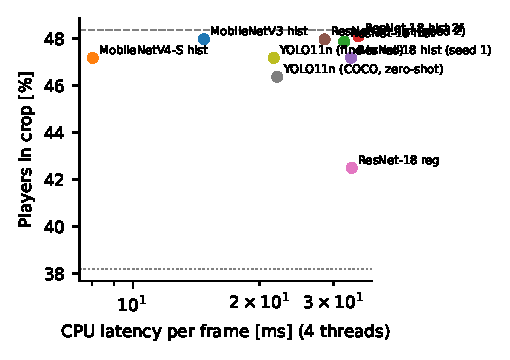
\includegraphics[width=\columnwidth]{figs/tradeoff.pdf}
\caption{Smoothed players in crop versus CPU latency (dashed: smoothed oracle, dotted: fixed centre).}
\label{fig:tradeoff}
\end{figure}

\subsection{Adding the ball: SN-Tracking-2023}
\textbf{Ball tracking.} Table~\ref{tab:ball} compares the two ball sources. The ResNet-18 heatmap network finds the ball within $38$\,px in $76.0\%$ of the ball-visible test frames from its single strongest peak and $77.2\%$ after tracking, with $71.1\%$ precision, although it is the most expensive component ($16$\,ms on GPU, $122$\,ms on CPU for a full $504{\times}896$ frame). The fine-tuned YOLO11n is two to four times faster, but its recall is only $50.4\%$ (precision $88.8\%$): it misses the ball in half of the frames. The tracker raises its recall to $60.5\%$ by bridging gaps, at the cost of precision. Static-overlay suppression slightly reduced recall on this test set ($77.2\%$ against $78.3\%$ without it, tracked ResNet-18), possibly because a ball that rests near one spot during set pieces is mistaken for an overlay; we keep it because a broadcast logo produced a false ball detection in a frame of an external broadcast clip we inspected (not measured).

\begin{table}[t]
\centering
\caption{Ball detection and tracking on the SN-Tracking-2023 test clips: recall / precision (\%) within $2\%$ of the frame width, from the strongest peak (raw) and after the tracker; coverage = frames with an estimate. Latency per $504{\times}896$ frame.}
\label{tab:ball}
\setlength{\tabcolsep}{3pt}
\begin{tabular}{lrrrrrrr}
\toprule
Ball source & GPU & CPU & \multicolumn{2}{c}{raw R/P} & \multicolumn{2}{c}{tracked R/P} & Cov.\\
 & [ms] & [ms] & & & & & [\%] \\
\midrule
ResNet-18 heatmap & 16 & 122 & 76.0 & 70.3 & 77.2 & 71.1 & 99.9 \\
YOLO11n & 8 & 34 & 50.4 & 88.8 & 60.5 & 69.6 & 80.0 \\
\bottomrule

\end{tabular}
\end{table}

\textbf{Crop policies.} Table~\ref{tab:sn} and Fig.~\ref{fig:sn} show the effect on the crop. A fixed centre crop already contains the ball in $53.0\%$ of the frames, because broadcast cameras keep it near the middle, but the crop of the densest group of players contains it in only $40.3\%$. Centring the window on the tracked ResNet-18 ball raises ball-in-crop to $88.0\%$ with $34.6\%$ of the players; adding the player histogram (ball + players) keeps $89.2\%$ of the balls and recovers $9$ points of player coverage ($43.6\%$), against a reference of $100\%$ and $48.5\%$. With ground-truth ball and predicted players the crop reaches $45.0\%$, so the learned player module accounts for $3.5$ of the $4.9$ points of missing player coverage, whereas the $11$-point ball-in-crop gap is due to the ball estimate. The YOLO11n pipeline covers more players ($46.7\%$) but loses the ball more often ($81.6\%$). A player module trained on SportsMOT and applied unchanged to SN-Tracking performs the same as the SN-trained one ($43.3\%$ against $43.6\%$ players in crop), indicating that the player-density task transfers between the two data sets.

\begin{table*}[t]
\centering
\caption{Crop policies on the 49 SN-Tracking-2023 test clips (12\,250 frames). Raw / smoothed (EMA $\alpha=0.6$, pan limit $5\%$ per sample) values; jitter in \% of frame width. Rows above the rule use ground truth. Systems are named ball source / player source / policy.}
\label{tab:sn}
\begin{tabular}{lrrrrrr}
\toprule
Policy & \multicolumn{2}{c}{Ball in crop [\%]} & \multicolumn{2}{c}{Players in crop [\%]} & \multicolumn{2}{c}{Jitter [\%]}\\
 & raw & smooth & raw & smooth & raw & smooth \\
\midrule
Fixed centre & 53.0 & 53.0 & 39.0 & 39.0 & 0.0 & 0.0 \\
Median of players (GT) & 40.9 & 40.8 & 49.3 & 49.1 & 1.1 & 0.8 \\
Ball-centred (GT ball) & 100.0 & 99.4 & 35.0 & 35.1 & 1.1 & 0.9 \\
Oracle (GT ball + players) & 100.0 & 98.3 & 48.5 & 44.4 & 2.1 & 1.4 \\
GT ball + predicted players & 100.0 & 98.9 & 45.0 & 43.8 & 2.1 & 1.4 \\
\midrule
ResNet-18 heatmap / SN-trained / players only & 40.3 & 40.3 & 57.8 & 56.1 & 2.8 & 1.5 \\
ResNet-18 heatmap / SN-trained / ball only (tracked) & 88.0 & 87.5 & 34.6 & 35.0 & 1.7 & 1.3 \\
ResNet-18 heatmap / SN-trained / ball + players (no tracker) & 86.4 & 88.1 & 44.0 & 42.9 & 6.0 & 2.0 \\
ResNet-18 heatmap / SN-trained / ball + players (tracked) & 89.2 & 88.1 & 43.6 & 42.7 & 2.2 & 1.4 \\
ResNet-18 heatmap / SportsMOT-trained / ball + players (tracked) & 88.9 & 87.9 & 43.3 & 42.5 & 2.2 & 1.4 \\
YOLO11n / YOLO11n / ball only (tracked) & 85.0 & 84.5 & 34.8 & 35.1 & 1.3 & 1.1 \\
YOLO11n / YOLO11n / ball + players (no tracker) & 71.4 & 70.8 & 50.3 & 46.6 & 6.5 & 2.3 \\
YOLO11n / YOLO11n / ball + players (tracked) & 81.6 & 80.1 & 46.7 & 44.5 & 3.1 & 1.8 \\
FB-style tiny (0.19M) / same network / ball only (tracked) & 86.2 & 86.5 & 34.1 & 34.5 & 2.0 & 1.4 \\
FB-style tiny (0.19M) / same network / ball + players (tracked) & 86.4 & 85.7 & 43.7 & 42.4 & 2.7 & 1.7 \\
FB-style ResNet-18 / same network / ball only (tracked) & 86.1 & 86.4 & 33.8 & 34.3 & 2.1 & 1.4 \\
FB-style ResNet-18 / same network / ball + players (tracked) & 87.1 & 86.3 & 43.4 & 42.0 & 2.8 & 1.7 \\
FB-style ResNet-18 v2 (2-frame, mined neg.) / same network / ball only (tracked) & 87.7 & 87.7 & 34.1 & 34.8 & 2.1 & 1.5 \\
FB-style ResNet-18 v2 (2-frame, mined neg.) / same network / ball + players (tracked) & 88.3 & 87.2 & 43.5 & 42.4 & 2.7 & 1.7 \\
\bottomrule

\end{tabular}
\end{table*}

\begin{figure}[t]
\centering
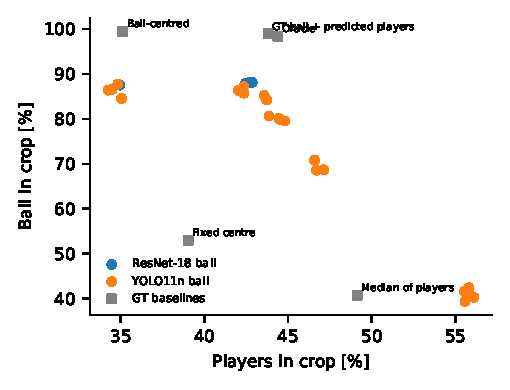
\includegraphics[width=\columnwidth]{figs/sn_scatter.pdf}
\caption{Ball in crop versus players in crop (smoothed) on SN-Tracking-2023 for the ground-truth baselines and all evaluated systems.}
\label{fig:sn}
\end{figure}

\textbf{Role of the tracker and of smoothing.} Without the tracker the ball + players policy follows single-frame peaks and jumps by $6.0\%$ of the frame width between samples; the tracker lowers raw jitter to $2.2\%$ and raises raw ball-in-crop from $86.4\%$ to $89.2\%$. After smoothing both variants contain the ball in $88.1\%$ of the frames and the jitter is $2.0\%$ against $1.4\%$, so the tracker mainly stabilises the estimate before smoothing. Smoothing costs about one point of ball-in-crop and one point of player coverage here, much less than for players alone, possibly because the ball trajectory is smoother than the player distribution.

\section{Discussion and Limitations}
\textbf{Proxy ground truth.} Neither data set contains a human-operated virtual camera. The SportsMOT oracle keeps the most players in view and the SN-Tracking oracle additionally keeps the ball in view; both are reasonable but imperfect stand-ins for what viewers care about, because a human editor would follow the play and would sometimes prefer fewer players in a tighter shot, or let the ball leave the frame briefly. The metrics should be read as agreement with an annotation-based rule, not as perceived quality, and we ran no user study.

\textbf{Scale.} Training used 12 videos (2\,801 frames) and ran for minutes per model on a single 4\,GB GPU. Validation on 3 videos was optimistic ($55\%$ raw for the histogram models) compared with the 15 test videos ($52\%$), which illustrates how variable the content is. Only the ResNet-18 histogram model has repeated seeds. Transfer to other broadcasters and camera styles was not evaluated quantitatively.

\textbf{Ball experiments.} The ball network was trained for only 18 minutes (10 epochs) and may be under-trained; the ball detectors are single-seed; ball-visible frames are $92\%$ of the test frames and frames without a visible ball are excluded from ball-in-crop; the static-overlay filter and the tracker use clip-level statistics or hand-set gates and are not causal in the first case. Full-frame ball inference at $504{\times}896$ is expensive on CPU ($122$\,ms), so real-time on-device use would need a smaller or tile-based ball model or a lower inference rate. Frames in the external-broadcast demonstration clip were inspected visually only.

\textbf{Metric and causality.} Players in crop counts a player once its box centre is inside the window and weights all players equally; goalkeepers and distant players count as much as those near the ball. The smoothing is causal, so no look-ahead is used, but we did not tune the smoothing parameters ($\alpha=0.5$, step limit $2\%$); a joint optimisation of the camera path would likely recover part of the 4-point cost.

\section{Conclusion}
Choosing a 9:16 crop from player positions is well within the reach of very small networks, and adding the ball makes the crop follow the play. A histogram-of-players head on a ResNet-18 or MobileNet backbone keeps about $52\%$ of players in view (raw) against $38\%$ for a fixed crop, and after smoothing performs on par with a fine-tuned YOLO11n pipeline and with the smoothed oracle, at 8--34\,ms per frame on CPU. Direct regression of the crop centre is not competitive. With a ResNet-18 ball heatmap, a small tracker and a ball-aware window rule, the crop contains the ball in $89\%$ of the visible frames on SN-Tracking-2023, against $53\%$ for a fixed centre crop, while still covering $43.6\%$ of the players; a fine-tuned YOLO11n loses the ball in about $1.7$ times as many frames. Future work should use a human-operated reference, per-player importance, causal tracking with a lighter ball model and a user study.

\begin{thebibliography}{10}
\bibitem{liu2006} F.~Liu and M.~Gleicher, ``Video retargeting: Automating pan and scan,'' in \emph{Proc. ACM Multimedia}, 2006.
\bibitem{giancola2018} S.~Giancola, M.~Amine, T.~Dghaily, and B.~Ghanem, ``SoccerNet: A scalable dataset for action spotting in soccer videos,'' in \emph{CVPR Workshops}, 2018.
\bibitem{cioppa2022} A.~Cioppa \emph{et~al.}, ``SoccerNet-Tracking: Multiple object tracking dataset and benchmark in soccer videos,'' in \emph{CVPR Workshops}, 2022.
\bibitem{cui2023} Y.~Cui \emph{et~al.}, ``SportsMOT: A large multi-object tracking dataset in multiple sports scenes,'' in \emph{ICCV}, 2023.
\bibitem{he2016} K.~He, X.~Zhang, S.~Ren, and J.~Sun, ``Deep residual learning for image recognition,'' in \emph{CVPR}, 2016.
\bibitem{howard2019} A.~Howard \emph{et~al.}, ``Searching for MobileNetV3,'' in \emph{ICCV}, 2019.
\bibitem{qin2024} D.~Qin \emph{et~al.}, ``MobileNetV4: Universal models for the mobile ecosystem,'' in \emph{ECCV}, 2024.
\bibitem{yolo11} G.~Jocher and J.~Qiu, ``Ultralytics YOLO11,'' 2024. [Online]. Available: \url{https://github.com/ultralytics/ultralytics}
\bibitem{zhou2019} X.~Zhou, D.~Wang, and P.~Kr\"ahenb\"uhl, ``Objects as points,'' arXiv:1904.07850, 2019.
\bibitem{huang2019} Y.-C. Huang \emph{et~al.}, ``TrackNet: A deep learning network for tracking high-speed and tiny objects in sports applications,'' in \emph{AVSS}, 2019.
\bibitem{lin2017} T.-Y. Lin, P. Goyal, R. Girshick, K. He, and P. Doll\'ar, ``Focal loss for dense object detection,'' in \emph{ICCV}, 2017.
\bibitem{loshchilov2019} I.~Loshchilov and F.~Hutter, ``Decoupled weight decay regularization,'' in \emph{ICLR}, 2019.
\end{thebibliography}

\end{document}
